\documentclass{beamer}

\usepackage[utf8]{inputenc}
\DeclareUnicodeCharacter{00A0}{ }%Permet d'éviter certains conflits de caractères invisibles
\usepackage{amssymb}            % Principaux symboles
%\usepackage{fontspec}
%\usepackage{xunicode}
%\usepackage{xltxtra}
\usepackage[frenchb]{babel}
%\defaultfontfeatures{Scale=MatchLowercase}
%\setmainfont[Mapping=tex-text,Ligatures={Common, Historical}]{Linux Libertine O}
%\setsansfont[Mapping=tex-text]{Linux Biolinum O}
%\setmonofont[Scale=0.75]{DejaVu Sans Mono}

%% Packages pour le texte
%\usepackage[misc,geometry]{ifsym}	% Police numéros battons
\usepackage{pifont}		% Police \ding
\usepackage{eurosym}		% Symbole de l'euro
\usepackage{soul}		% Souligner
\usepackage{enumerate}		% Listes
\usepackage{verbatim}		% Codes source
\usepackage{moreverb}		%	et listings
\usepackage{textcomp}
\usepackage{multicol}

%% Packages pour les tableaux
\usepackage{array}		% Outils supplémentaires
\usepackage{multirow}		% Colonnes multiples
\usepackage{tabularx}		% Largeur totale donnée
\usepackage{longtable}		% Sur plusieurs pages

%% Les packages pour les dessins
\usepackage{graphicx}		% Insertion de figures
%\usepackage{picins}		% Dans un paragraphe
\usepackage{epic}		% Capacités graphiques
\usepackage{eepic}		% 	étendues
\usepackage{afterpage}		% Voir page 69
\usepackage{rotating}		% Tourner du texte
\usepackage{caption}		% Légendes
% \addto\captionsfrench{\def\figurename{}}

%% Packages pour les maths
\usepackage{amsmath}		% Commandes essentielles
\usepackage{amssymb}		% Principaux symboles
\usepackage{mathrsfs}		% Police calligraphique
\usepackage{theorem}		% Théorèmes
%\usepackage{tikz}		% Courbes
\usepackage{esvect}            % Vecteurs
%\usetikzlibrary{shapes,arrows,shadows}
\usepackage{pgf}
%\usetikzlibrary{arrows}
% Packages pour la physique
%\usepackage{sistyle}		% Unités
\usepackage[version=3]{mhchem}	% Formules chimiques
\usepackage{etex}
%\usepackage{m-pictex,m-ch-en}

%\usepackage{media9}
\usepackage{multimedia}		% Vidéos dans la présentation
%\usepackage{movie15}

%Ajout d'images de fond:
\usepackage{eso-pic}
\usepackage{wallpaper}

\usepackage{ccicons}		% Licence creativecommons
\usepackage{xcolor,colortbl}

%\SIdecimalsign{,}


\AtBeginSection[]
{
  \begin{frame}
    \frametitle{Sommaire}
    \begin{multicols}{2}
      {\small
				\setcounter{tocdepth}{2}
        \tableofcontents[currentsection, hideothersubsections]}
    \end{multicols}
  \end{frame}
}

\usetheme{Warsaw}

\usepackage{tikz}
\usetikzlibrary{arrows,automata}
\usepackage{fancyvrb}
\usepackage[french,onelanguage]{algorithm2e}

\useoutertheme{infolines}
\setbeamersize{text margin left=1cm,text margin right=1cm}

\title{Analyseur syntaxique}
\subtitle{Rapport de projet VISI\_201}
\author{Porteries Tristan}

\begin{document}

\begin{frame}
  \titlepage
\end{frame}

\begin{frame}
    \frametitle{Sommaire}
    \begin{multicols}{2}
      {
% 		\setcounter{tocdepth}{1}
        \tableofcontents
      }
    \end{multicols}
\end{frame}

\begin{frame}{Introduction}
 Objectifs d'un analyseur syntaxique~:
 \begin{itemize}
  \item déterminer l'existence d'une chaîne selon une grammaire~;
  \item reporter des erreurs~;
  \item construire un arbre abstrait de syntaxe.
 \end{itemize}
\end{frame}

\begin{frame}[fragile]
	\begin{columns}
		\begin{column}{0.5\textwidth}
			\begin{center}
				\begin{BVerbatim}
5 + 2 - 3
				\end{BVerbatim}
			\end{center}
		\end{column}
		\begin{column}{0.5\textwidth}
			\begin{tikzpicture}[sibling distance=5em, every node/.style = {shape=rectangle, rounded corners, draw, align=center,
    top color=white, bottom color=blue!20}]]
				\node {+}
					child { node {5} }
					child { node {-} 
					child { node {2} }
					child { node {3} }
				};
			\end{tikzpicture}
		\end{column}
	\end{columns}
\end{frame}

\section{Grammaires non-contextuelles}

\begin{frame}
 $$ G = (V, A, S, P) $$
 
 \begin{itemize}
  \item $V$ : ensemble des non-terminaux.
  \item $A$ : ensemble des terminaux.
  \item $S$ : non-terminal axiome, $S \in V$.
  \item $P$ : ensemble des productions, $P \subset V \times (A \cup V)^*$.
 \end{itemize}
\end{frame}

\begin{frame}[fragile]
	Les grammaires pouvant produire des arbres de dérivations sont ambiguës.

	$$E \rightarrow E + E$$
	$$E \rightarrow id $$

	\begin{center}
		\begin{BVerbatim}
5 + 3 + 2
		\end{BVerbatim}
	\end{center}

	\begin{columns}
		\begin{column}{0.5\textwidth}
			\begin{center}
				\begin{tikzpicture}[sibling distance=3em, every node/.style = {shape=rectangle, rounded corners, draw, align=center,
    top color=white, bottom color=blue!20}]]
					\node {+}
						child { node {5} }
						child { node {+} 
						child { node {3} }
						child { node {2} }
					};
				\end{tikzpicture}
			\end{center}
		\end{column}
		\begin{column}{0.5\textwidth}
			\begin{center}
				\begin{tikzpicture}[sibling distance=3em, every node/.style = {shape=rectangle, rounded corners, draw, align=center,
    top color=white, bottom color=blue!20}]]
					\node {+}
						child { node {+} 
						child { node {5} }
						child { node {3} }}
						child { node {2} };
				\end{tikzpicture}
			\end{center}
		\end{column}
	\end{columns}

	Toléré pour les opérateurs commutatifs.

\end{frame}


\begin{frame}[fragile]
 $$ S \rightarrow aSb $$
 $$ S \rightarrow \epsilon $$

 Une dérivation d'un non-terminal selon une production mène à une proto-phrase ou phrase.

		\begin{verbatim}
aabb
		\end{verbatim}

 $$ S \rightarrow aSb$$
 $$ S \rightarrow aaSbb$$
 $$ S \rightarrow aabb$$
 $$ \boxed{S \xrightarrow{*} aabb}$$
\end{frame}


\section{Hiérachie de Chomsky}

\begin{frame}
	\begin{center}
		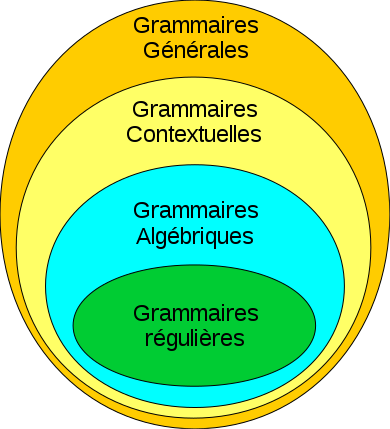
\includegraphics[width=5cm]{Images/chomsky.png} \\
		\begin{tabular}{|c|c|}
			\hline
				Grammaires contextuelles & $\alpha A \beta \rightarrow \alpha \gamma \beta $ \\
			\hline
				Grammaires algébriques & $A \rightarrow \gamma $ \\
			\hline
				Grammaire régulières & $ A \rightarrow a B, A \rightarrow a $ \\
			\hline
		\end{tabular}
	\end{center}
\end{frame}

\section{Analyseur lexical}

\begin{frame}
 Analyse de la chaine d'entrée pour reconnaitre des lexèmes.
 Utilisation d'expression pour décrire des grammaires linéaire.

 Soit $x$ et $y$ appartenant au langage~: \\
 \begin{center}
	\begin{tabular}{|l|c|c|}
		\hline
		Opération & Notation & Exemple \\
		\hline
		Concaténation & $xy$ & $\{ab\}$ \\
		\hline
		Union & $x|y$ & $\{a, b\}$ \\
		\hline
		Étoile Kleene & $(x|y)*$ & $\{\epsilon, a, b, ab, ba, aa, bb, ...\}$ \\
		\hline
	\end{tabular}
 \end{center}

 Limitation : $a^nb^n$
\end{frame}

\subsection{Automates finis}

\begin{frame}
	Théorème de Kleene~: l'ensemble des langages rationnels sur un alphabet A est exactement l'ensemble des langages sur A reconnaissables par automate fini.
	\begin{figure}[!c]
	 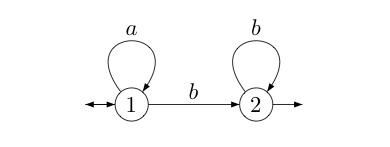
\includegraphics[width=7cm]{Images/Automate-synchronise.png}
	 \caption{Automate reconnaissant le langage $a^*b^*$}
	\end{figure}

\end{frame}

\section{Analyseur syntaxique}

\subsection{Backus-Naur Form}

\begin{frame}[fragile]
 Description de règles d'analyse (productions)~:

 \begin{center}
	$A \rightarrow aAb$ \\
	\begin{BVerbatim}
<A> ::= a <A> b
	\end{BVerbatim}
 \end{center}
\end{frame}

\subsection{Automates à piles}

\begin{frame}
 
\end{frame}

\subsection{Analyseur LL}

\begin{frame}
 Dérivation de l'axiome à partir de la gauche, si les dérivations mènent à la phrase d'entrée~: accepter la phrase.

 Si $S \xrightarrow{*} \omega$ accepter $\omega$

 \begin{center}
  $S \rightarrow aAb$ \\
  $S \rightarrow \epsilon$ \\
 \end{center}

 $\omega = aabb$
 \begin{enumerate}
  \item $S$
  \item $aAb$
  \item $aaAbb$
  \item $aabb$
 \end{enumerate}
\end{frame}

\begin{frame}
	Contrainte de récursivité gauche des productions.

	$$ A \rightarrow A\alpha $$ 
	$$ A \rightarrow \beta $$

	Suppression de la récursivité gauche~:
	$$ A \rightarrow \beta A' $$
	$$ A' \rightarrow \alpha A' $$
	$$ A' \rightarrow \epsilon $$

\end{frame}

\begin{frame}
\begin{algorithm}[H]
 initialiser une pile contenant S\;
 soit C le premier lexème\;
 \While{la pile est non-vide} {
  soit T le sommet de la pile\;
  \eIf{T est non-terminal} {
		choisir une production P\;
		dépiler le sommet de la pile\;
		empiler la partie droite de P\;
   }{
   \If{T = C} {
			dépiler le sommet de la pile\;
			passer C au lexème suivant\;
		}
		\Else {
			erreur\;
		}
	 }
 }
 \caption{Algorithme LL à pile}
\end{algorithm}
\end{frame}

\begin{frame}
	\begin{center}
		\begin{tabular}{|l|l|c|}
			\hline
			Pile & Entrée & Opération \\
			\hline
			$S$ & aabb & \\
			$aSb$ & aabb & dériver $S \rightarrow aSb$ \\
			$Sb$ & abb & valider $a$ \\
			$aSbb$ & abb & dériver $S \rightarrow aSb$ \\
			$Sbb$ & bb & valider $a$ \\
			$bb$ & bb & dériver $S \rightarrow \epsilon$ \\
			$b$ & b & valider $b$ \\
			& & valider $b$ \\
			\hline
		\end{tabular}
	\end{center}
\end{frame}

\begin{frame}
 Comment choisir la production à dériver ?

 Utilisation d'un symbole de prévision~: analyseur LL(1). Construction d'une table associant non-terminal, lexème à une production.

 Limitation~: seul les grammaires où toutes les productions d'un non-terminal n'ont pas les mêmes terminaux préfixes.

 $$ A \rightarrow a \gamma $$
 $$ A \rightarrow b \gamma $$
\end{frame}


\subsection{Analyseur LR}

\begin{frame}
	Lire l'entrée depuis la gauche, reconnaître des production et réduire (décalage / réduction).

	\begin{center}
		\begin{tabular}{|l|l|c|}
			\hline
			Pile & Entrée & Opération \\
			& $aabb$ &  \\
			$a$ & $abb$ & décaler \\
			$aa$ & $bb$ & décaler \\
			$aab$ & $b$ & décaler \\
			$aA$ & $b$ & réduire $A \rightarrow ab$ \\
			$aAb$ & & décaler \\
			$A$ & & réduire $A \rightarrow aAb$ \\
			\hline
		\end{tabular}
	\end{center}

	Avantage~: pas de récursivité.

	$$ A \rightarrow ab$$
	$$ A \rightarrow aAb $$

\end{frame}

\begin{frame}
	Reconnaître une partie droite de production n'est pas forcement un manche.

	$$ A \rightarrow aA $$
	$$ A \rightarrow a $$

	$\omega = aa$
	\begin{center}
		\begin{tabular}{|l|l|c|}
			\hline
			Pile & Entrée & Opération \\
			& $aa$ &  \\
			$a$ & $a$ & décaler \\
			$A$ & $a$ & réduire $A \rightarrow a$ \\
			$Aa$ & & décaler \\
			\hline
		\end{tabular}
	\end{center}

\end{frame}


\begin{frame}
 Construction d'items de production, état de l'analyse~:

 $$ A \rightarrow \bullet \alpha A \beta $$
 $$ A \rightarrow \alpha \bullet A \beta $$
 $$ A \rightarrow \alpha A \bullet \beta $$
 $$ A \rightarrow \alpha A \beta \bullet $$

 Détection d'une potentielle réduction, un manche~:
 $$ A \rightarrow \alpha A \beta \bullet $$
\end{frame}

\begin{frame}
	Utilisation d'une grammaire augmentée $G'$ d'éléments $G$ et d'axiome $S'$ avec la production~:
	$$ S' \rightarrow S$$
	Acceptation de la chaîne d'entrée lors de la réduction $ S' \rightarrow S$.
\end{frame}


\begin{frame}
	Opération sur les ensembles d'items~:
	\begin{itemize}
		\item $Fermeture(E)$~: Soit $(A \rightarrow \gamma \bullet B) \in E$ tous les items de la forme $B \rightarrow \bullet \gamma$ et $E$.
		\item $Transition(E, X)$~: $Fermeture$ de l'ensemble des items $A \rightarrow \alpha X \bullet \beta$ si $A \rightarrow \alpha \bullet X \beta$ est présent dans E.
	\end{itemize}
\end{frame}

\begin{frame}
	$$ S \rightarrow aSb $$
	$$ S \rightarrow ab $$

	$Fermeture(\{S' \rightarrow \bullet S\}) = \{
	S' \rightarrow \bullet S,
	S \rightarrow \bullet aSb,
	S \rightarrow \bullet ab
	\} = I_0$ \\
	$Transition(I_0, S) = \{
	S' \rightarrow S \bullet
	\} = I_1$ \\
	$Transition(I_0, a) = \{
	S \rightarrow a \bullet Sb,
	S \rightarrow a \bullet b,
	S \rightarrow \bullet aSb,
	S \rightarrow \bullet ab
	\} = I_2$ \\
	$Transition(I_2, S) = \{
	S \rightarrow aS \bullet b
	\} = I_3$ \\
	$Transition(I_2, a) = I_2$ \\
	$Transition(I_2, b) = \{
	S \rightarrow ab \bullet
	\} = I_4$ \\
	$Transition(I_3, b) = \{
	S \rightarrow aSb \bullet
	\} = I_5$
\end{frame}

\begin{frame}
	La collection des ensembles $Transition$ et $Fermeture$ est appelé collection canonique LR.

	Utilisation d'un automate comme pour l'analyseur LL, chaque état est un ensemble de la collection.
\end{frame}

\begin{frame}
	\begin{center}
		\begin{tikzpicture}[->,>=stealth',shorten >=1pt,auto,node distance=2cm, semithick]
			\node[initial, state] (0) {$I_0$};
			\node[state] (1) [right of=0] {$I_1$};
			\node[state] (2) [below of=0] {$I_2$};
			\node[state] (3) [right of=2] {$I_3$};
			\node[state] (4) [below of=2] {$I_4$};
			\node[state] (5) [right of=3] {$I_5$};

			\path
				(0) edge node {$S$} (1)
				(0) edge node {$a$} (2)
				(2) edge node {$S$} (3)
				(3) edge node {$b$} (5)
				(2) edge node {$b$} (4)
				(2) edge [loop left] node {$a$} (2)
			;
		\end{tikzpicture}
	\end{center}
\end{frame}

\begin{frame}
\begin{center}
\scalebox{0.8} {
\begin{algorithm}[H]
 initialiser une pile vide\;
 soit $I_0$ et $I$ l'ensemble $Fermeture(\{S' \rightarrow \bullet S\})$\;
 soit $C$ le premier lexème\;
 \While{la pile n'est pas $\{S\}$} {
	soit $T$ l'ensemble $Transition(I, C)$\;
	\eIf{$T$ non vide} {
		empiler $C$ sur la pile\;
		passer $C$ au lexème suivant\;
		passer $I$ à $T$\;
	}
	{
		\If {$T$ contient un item $A \rightarrow \gamma \bullet$} {
			remplacer le sommet de la pile\;
			initialiser $I$ à $I_0$
		}
		\Else {
			erreur\;
		}
	}
 }
 \caption{Algorithme LR}
\end{algorithm}
}
\end{center}
\end{frame}


\section{Arbre abstrait}

\begin{frame}[fragile]
	\begin{center}
		\begin{tikzpicture}[sibling distance=10em, every node/.style = {shape=rectangle, rounded corners, draw, align=center,
			top color=white, bottom color=blue!20}]]
			\node {+}
				child { node {5} }
				child { node {-} 
				child { node {2} }
				child { node {3} }
			};
		\end{tikzpicture}
	\end{center}
	Les feuilles sont des opérandes, les autres nœuds des opérateurs.
\end{frame}

\subsection{Arbre de dérivation}

\begin{frame}[fragile]
	$$ E \rightarrow id\ E'$$
	$$ E' \rightarrow op\ id\ E'$$
	$$ E' \rightarrow \epsilon $$
	\begin{center}
		\scalebox{0.65}{
			\begin{tikzpicture}[sibling distance=6em, every node/.style = {shape=rectangle, rounded corners, draw, align=center,
			top color=white, bottom color=blue!20}]]
			\node {E}
				child { node {5} }
				child { node {E'}
					child { node {+} }
					child { node {2} }
					child { node {E'}
						child { node {-}}
						child { node {3}}
						child { node {E'}
							child { node {$\epsilon$} }
						}
					}
				}
			;
			\end{tikzpicture}
		}
	\end{center}
	Arbre des dérivations successives, les feuilles sont des terminaux, les autres nœuds des non-terminaux, la racine est l'axiome.
\end{frame}

\subsection{Grammaire attribuée}

\begin{frame}
 Associer à chaque production des règles pour construire les nœuds de l'arbre abstrait en fonction des nœuds de l'arbre de dérivation.
\end{frame}

\subsubsection{Attributs synthétisés}

\begin{frame}
 Attributs dépendant des nœuds fils d'un nœud de dérivation ou de lui même.
 
	\begin{align}
		E \rightarrow id\ E' \Longrightarrow& E.noeud = E'.noeud; \\
		E'_1 \rightarrow id\ op\ E'_2 \Longrightarrow& E'_1.noeud = noeud(op.val); \\
		&E'_1.noeud.ajouter(E'_2.noeud); \\
		E' \rightarrow \epsilon \Longrightarrow& E'.noeud = noeud();
	\end{align}
\end{frame}

\subsubsection{Attributs hérités}

\begin{frame}
 Attributs dépendant des nœuds parents.

 \begin{align}
	E \rightarrow id\ E' &\Longrightarrow E'.noeud.ajouter(noeud(id.val)) \\
  E'_1 \rightarrow id\ op\ E'_2 &\Longrightarrow E'_2.noeud.ajouter(noeud(id.val))
 \end{align}
\end{frame}

\begin{frame}[fragile]
	\begin{center}
		\begin{tikzpicture}[sibling distance=6em, BoxStyle/.style = {shape=rectangle, rounded corners, draw, align=center,top color=white, bottom color=blue!20}]]
			\node[BoxStyle] (E1) {E}
				child { node[BoxStyle] (id1) {5} }
				child { node[BoxStyle] (E2) {E'}
					child { node[BoxStyle] (op1) {+} }
					child { node[BoxStyle] (id2) {2} }
					child { node[BoxStyle] (E3) {E'}
						child { node[BoxStyle] (op2) {-}}
						child { node[BoxStyle] (id3) {3}}
						child { node[BoxStyle] (E4) {E'}
							child { node[BoxStyle] (eps) {$\epsilon$} }
						}
					}
				}
			;

			\path[->,draw=orange,thick]
				(E2) edge [bend right] node {$(1)$} (E1)
				(op1) edge [bend left] node {$(2)$} (E2)
				(op2) edge [bend left] node {$(2)$} (E3)
				(E3) edge [bend right] node {$(3)$} (E2)
				(E4) edge [bend right] node {$(3)$} (E3)
				(id1) edge node {$(5)$} (E2)
				(id2) edge node {$(6)$} (E3)
				(id3) edge node {$(6)$} (E4)
			;
		\end{tikzpicture}
	\end{center}
\end{frame}


\section{Implémentation}

\subsection{Usage}

\begin{frame}
 
\end{frame}


\end{document}
